\documentclass[tikz,border=8pt]{standalone}
\usepackage{amsmath,amssymb}
\usetikzlibrary{arrows.meta,automata,positioning,quotes}
\begin{document}
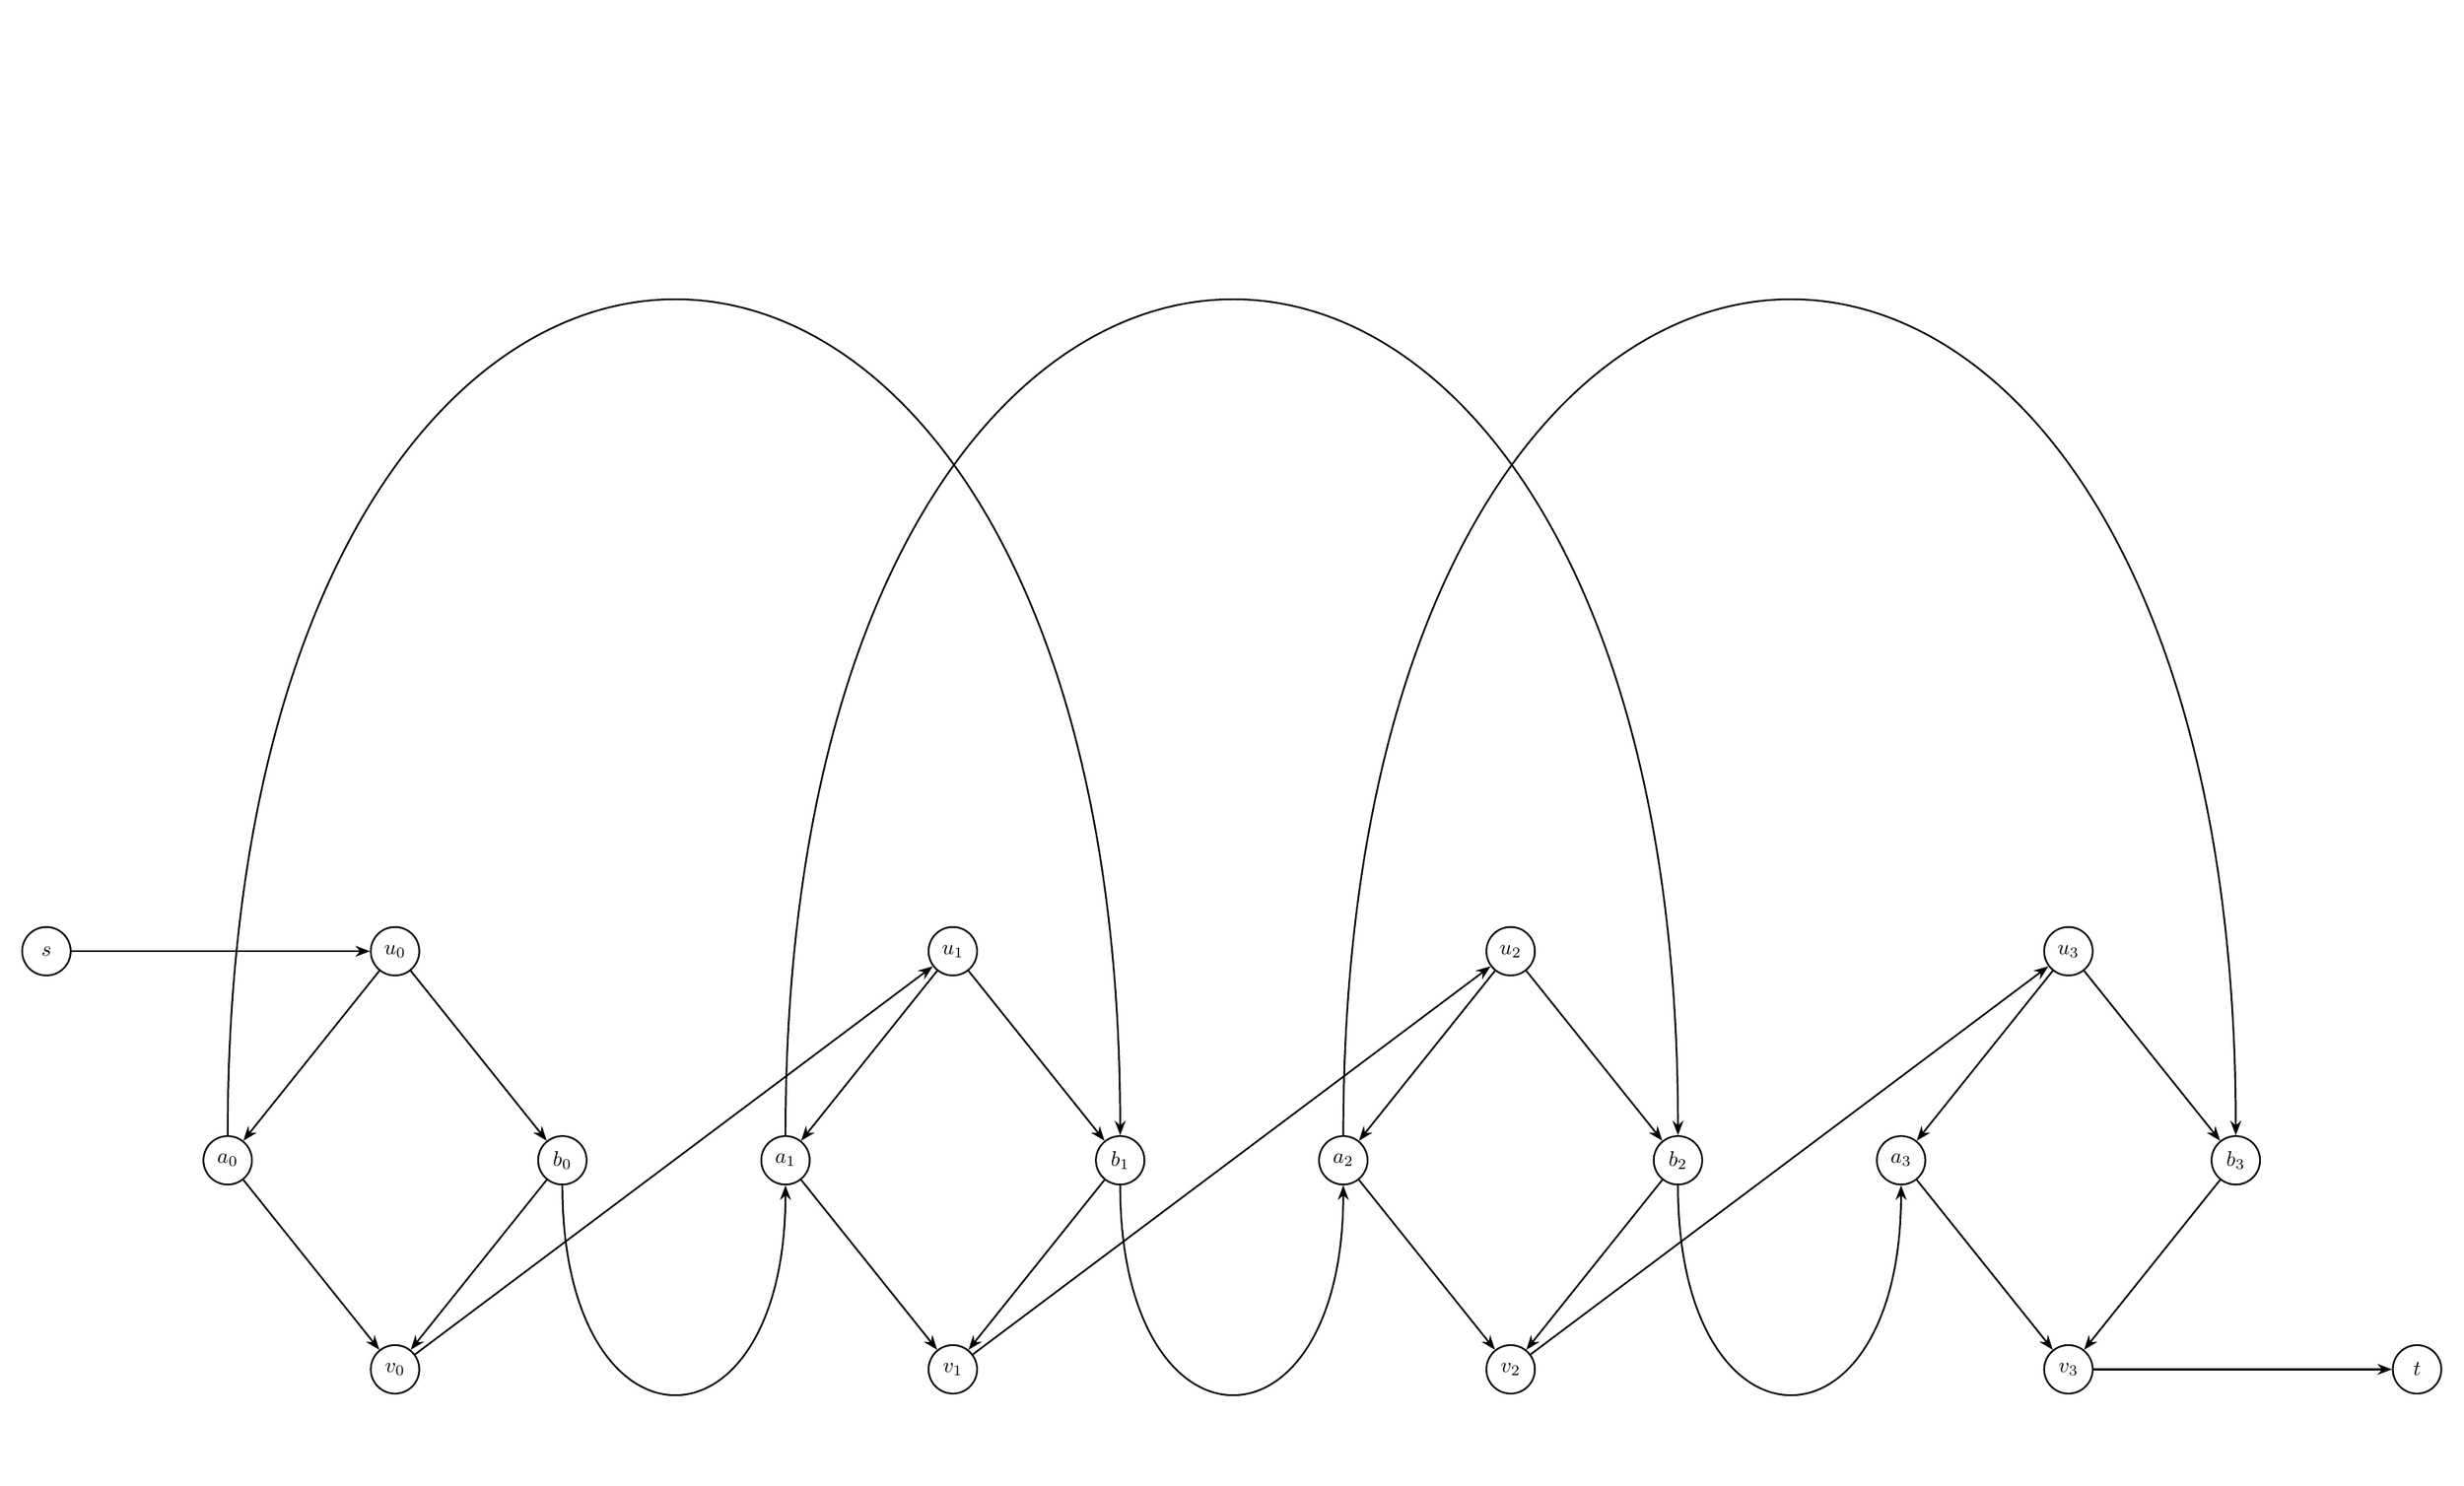
\begin{tikzpicture}[x=1cm,y=1cm]
\tikzset{
  graphnode/.style={circle,draw,thick,minimum size=8mm,inner sep=1pt,font=\sffamily},
  directed/.style={-{Stealth[length=2.4mm]},thick},
  undirected/.style={thick}
}
\node[graphnode] (n_s) at (-7.55,3.45) {$s$};
\node[graphnode] (n_u_0) at (-1.80,3.45) {$u_0$};
\node[graphnode] (n_v_0) at (-1.80,-3.45) {$v_0$};
\node[graphnode] (n_a_0) at (-4.56,0.00) {$a_0$};
\node[graphnode] (n_b_0) at (0.96,0.00) {$b_0$};
\node[graphnode] (n_u_1) at (7.40,3.45) {$u_1$};
\node[graphnode] (n_v_1) at (7.40,-3.45) {$v_1$};
\node[graphnode] (n_a_1) at (4.64,0.00) {$a_1$};
\node[graphnode] (n_b_1) at (10.16,0.00) {$b_1$};
\node[graphnode] (n_u_2) at (16.60,3.45) {$u_2$};
\node[graphnode] (n_v_2) at (16.60,-3.45) {$v_2$};
\node[graphnode] (n_a_2) at (13.84,0.00) {$a_2$};
\node[graphnode] (n_b_2) at (19.36,0.00) {$b_2$};
\node[graphnode] (n_u_3) at (25.80,3.45) {$u_3$};
\node[graphnode] (n_v_3) at (25.80,-3.45) {$v_3$};
\node[graphnode] (n_a_3) at (23.04,0.00) {$a_3$};
\node[graphnode] (n_b_3) at (28.56,0.00) {$b_3$};
\node[graphnode] (n_t) at (31.55,-3.45) {$t$};
\draw[directed] (n_u_0) -- (n_a_0);
\draw[directed] (n_u_0) -- (n_b_0);
\draw[directed] (n_a_0) -- (n_v_0);
\draw[directed] (n_b_0) -- (n_v_0);
\draw[directed] (n_u_1) -- (n_a_1);
\draw[directed] (n_u_1) -- (n_b_1);
\draw[directed] (n_a_1) -- (n_v_1);
\draw[directed] (n_b_1) -- (n_v_1);
\draw[directed] (n_u_2) -- (n_a_2);
\draw[directed] (n_u_2) -- (n_b_2);
\draw[directed] (n_a_2) -- (n_v_2);
\draw[directed] (n_b_2) -- (n_v_2);
\draw[directed] (n_u_3) -- (n_a_3);
\draw[directed] (n_u_3) -- (n_b_3);
\draw[directed] (n_a_3) -- (n_v_3);
\draw[directed] (n_b_3) -- (n_v_3);
\draw[directed] (n_s) -- (n_u_0);
\draw[directed] (n_v_0) -- (n_u_1);
\draw[directed] (n_v_1) -- (n_u_2);
\draw[directed] (n_v_2) -- (n_u_3);
\draw[directed] (n_v_3) -- (n_t);
\draw[directed] (n_a_0) to[out=90,in=90,looseness=3.2] (n_b_1);
\draw[directed] (n_b_0) to[out=-90,in=-90,looseness=3.2] (n_a_1);
\draw[directed] (n_a_1) to[out=90,in=90,looseness=3.2] (n_b_2);
\draw[directed] (n_b_1) to[out=-90,in=-90,looseness=3.2] (n_a_2);
\draw[directed] (n_a_2) to[out=90,in=90,looseness=3.2] (n_b_3);
\draw[directed] (n_b_2) to[out=-90,in=-90,looseness=3.2] (n_a_3);
\end{tikzpicture}
\end{document}
